\section{CoreSets Erzeugen}

CoreSets sind Räume mit einer Anhäufung mehrerer Punkte. Sie werden durch die frei wählbaren Parameter des Algorithmus, die vom
DBSCAN-Algorithmus inspiriert wurden \cite{7022654}, berechnet: $\epsilon$ und $\tau$. Ein
Referenzpunkt $P_{i}$ in
einem Subspace S ist genau dann mit einem anderen Punkt $P_{j}$ in S benachbart ($N^{S}(P_{i})$),
wenn $dist(P_{i}^{S}, P_{j}^{S})$ < $\epsilon$ und $P_{i} \neq P_{j}$. Außerdem muss gelten,
dass
$|N^{S}(P_{i})| >= \tau$. Ein CoreSet besteht also aus mindestens $\tau$ Punkten, die jeweils maximal $\epsilon$ voneinander entfernt sind.
CoreSets können Schnittpunkte in gemeinsamen Punkten bilden.

\begin{figure}[h]
    \centering
    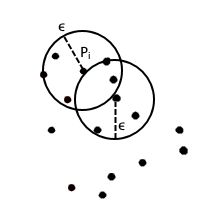
\includegraphics[width=0.5\textwidth]{SUBSCALE_nachbarschaft}
    \caption[Corset Erzeugung]{CoreSet Erzeugung}
    \label{img:CoresetsErzeugen}
\end{figure}


Auf diese Weise werden für jede Dimension CoreSets gebildet.